\subsection{Flyweight}

\subsubsection{Objetivo}

Suportar um grande número de objetos de tamanho reduzido através da partilha de estado entre eles.

\subsubsection{Motivação}

Considere-se por exemplo um editor de texto que necessita de manter a informação aos caracteres existentes num documento. Uma solução seria ter um objeto por caracter, mas isso seria inviável em termos de memória. O padrão Flyweight fornece um mecanismo para contornar esta limitação.

Um flyweight é um objeto partilhado que pode ser utilizado em múltiplos contextos simultaneamente. O conceito chave é a distinção entre estado intrínseco (guardado no flyweight, partilhado) e extrínseco (passado como parâmetro pelos clientes).

Usando este padrão passaríamos a ter a seguinte estrutura:

\centerline{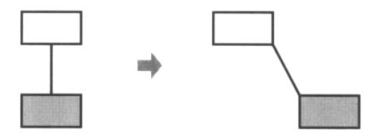
\includegraphics[scale=.7]{img/flyweight/motivation.png}}

Neste caso temos um flyweight para cada letra do alfabeto, responsável por guardar o código do caracter, e quando um cliente necessitar de desenhar uma dada letra recorre ao respetivo flyweight indicando a localização e a fonte pretendidas.

\subsubsection{Aplicação}

Usar quando:
\begin{itemize}
\item a aplicação usa um grande número de objetos;
\item é necessário reduzir a quantidade de objetos em memória;
\item uma grande parte do estado do objeto pode ser partilhada;
\item é possível substituir vários grupos de objetos por um número bem menor de objetos se o estado extrínseco for removido.
\end{itemize}

\subsubsection{Estrutura}

\centerline{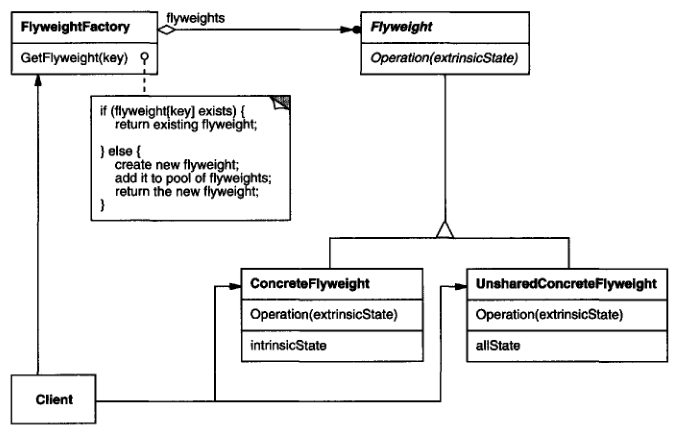
\includegraphics[scale=.7]{img/flyweight/structure1.png}}

O seguinte diagrama demonstra como os flyweights são partilhados:

\centerline{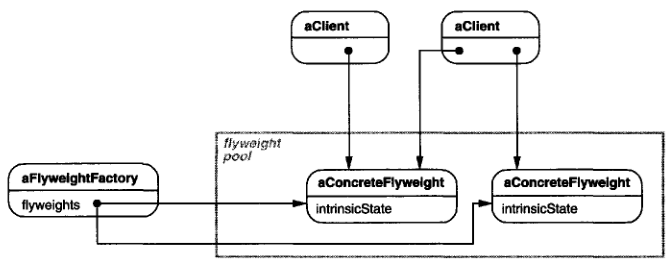
\includegraphics[scale=.7]{img/flyweight/structure2.png}}

\subsubsection{Participantes}
\begin{itemize}
\item Flyweight (Glyph), declara uma interface a partir da qual os flyweights recebem e manipulam o estado extrínseco
\item ConcreteFlyweight (Character), implementa a interface Flyweight e adiciona o estado intrínseco
\item UnsharedConcreteFlyweight (Row, Column), não partilha estado, tipicamente agrega coleções de objetos ConcreteFlyweight
\item FlyweightFactory, cria e gere objetos flyweight
\item Client, mantém as referências para os flyweights e define o seu estado extrínseco
\end{itemize}

\subsubsection{Colaborações}

\begin{itemize}
\item O estado intrínseco é guardado no objeto ConcreteFlyweight e o estado extrínseco é guardado ou calculado por objetos Client.
\item Os clientes não devem criar instâncias ConcreteFlyweight, mas obtê-las a partir de uma FlyweightFactory.
\end{itemize}

\subsubsection{Consequências}
\begin{itemize}
\item As operações associadas à gestão do estado extrínseco podem ter impacto no desempenho.
\item Quantos mais flyweights forem partilhados e quanto maior for o estado partilhado, maior será a poupança de memória.
\item Caso se pretenda combinar este padrão com o padrão Composite, as referências para os pais têm de ser passadas como parte do estado extrínseco.
\end{itemize}

\subsubsection{Implementação}
\begin{itemize}
\item O estado extrínseco deve ser reduzido, caso contrário não será possível tirar partido das vantagens pretendidas.
\item Se o número de flyweights não for fixo e pequeno, pode ser necessário efetuar a gestão dos objetos partilhados por forma a reduzir o impacto ao nível do desempenho e uso de memória.
\end{itemize}